\documentclass{article}\usepackage[]{graphicx}\usepackage[]{color}
%% maxwidth is the original width if it is less than linewidth
%% otherwise use linewidth (to make sure the graphics do not exceed the margin)
\makeatletter
\def\maxwidth{ %
  \ifdim\Gin@nat@width>\linewidth
    \linewidth
  \else
    \Gin@nat@width
  \fi
}
\makeatother

\definecolor{fgcolor}{rgb}{0.345, 0.345, 0.345}
\newcommand{\hlnum}[1]{\textcolor[rgb]{0.686,0.059,0.569}{#1}}%
\newcommand{\hlstr}[1]{\textcolor[rgb]{0.192,0.494,0.8}{#1}}%
\newcommand{\hlcom}[1]{\textcolor[rgb]{0.678,0.584,0.686}{\textit{#1}}}%
\newcommand{\hlopt}[1]{\textcolor[rgb]{0,0,0}{#1}}%
\newcommand{\hlstd}[1]{\textcolor[rgb]{0.345,0.345,0.345}{#1}}%
\newcommand{\hlkwa}[1]{\textcolor[rgb]{0.161,0.373,0.58}{\textbf{#1}}}%
\newcommand{\hlkwb}[1]{\textcolor[rgb]{0.69,0.353,0.396}{#1}}%
\newcommand{\hlkwc}[1]{\textcolor[rgb]{0.333,0.667,0.333}{#1}}%
\newcommand{\hlkwd}[1]{\textcolor[rgb]{0.737,0.353,0.396}{\textbf{#1}}}%

\usepackage{framed}
\makeatletter
\newenvironment{kframe}{%
 \def\at@end@of@kframe{}%
 \ifinner\ifhmode%
  \def\at@end@of@kframe{\end{minipage}}%
  \begin{minipage}{\columnwidth}%
 \fi\fi%
 \def\FrameCommand##1{\hskip\@totalleftmargin \hskip-\fboxsep
 \colorbox{shadecolor}{##1}\hskip-\fboxsep
     % There is no \\@totalrightmargin, so:
     \hskip-\linewidth \hskip-\@totalleftmargin \hskip\columnwidth}%
 \MakeFramed {\advance\hsize-\width
   \@totalleftmargin\z@ \linewidth\hsize
   \@setminipage}}%
 {\par\unskip\endMakeFramed%
 \at@end@of@kframe}
\makeatother

\definecolor{shadecolor}{rgb}{.97, .97, .97}
\definecolor{messagecolor}{rgb}{0, 0, 0}
\definecolor{warningcolor}{rgb}{1, 0, 1}
\definecolor{errorcolor}{rgb}{1, 0, 0}
\newenvironment{knitrout}{}{} % an empty environment to be redefined in TeX

\usepackage{alltt}
\usepackage{amsmath,amsfonts,bm,fullpage,multirow,animate,subcaption,graphicx,caption}
\usepackage{natbib,tikz}
\bibliographystyle{abbrvnat}
\DeclareMathOperator*{\argmax}{arg\,max}
\newcommand{\ProjMean}{{\widehat{\bm S}_{E}}}
\newcommand{\ProjMedian}{{\widehat{\bm S}_{1}}}
\newcommand{\HuberMean}{{\widehat{\bm S}_H}}
\newcommand{\WeightMean}{{\widehat{\bm S}_W}}
\newcommand{\TrimMean}{{\widehat{\bm S}_T}}
\newcommand{\WinzMean}{{\widehat{\bm S}_Z}}
\newcommand{\GeomMean}{{\widehat{\bm S}_{R}}}
\newcommand{\R}{{\mathbb{R}}}
\newcommand{\qest}{{\hat{\bm q}}}
\newcommand{\Sest}{{\widehat{\bm S}}}
\IfFileExists{upquote.sty}{\usepackage{upquote}}{}
\begin{document}

\begin{center}
\Large{\bf Robust Topics in $SO(3)$}
\end{center}
\normalsize
This is a summary of the material related to robustness for $SO(3)$ data.  A detailed account of outlier detection for circular and spherical data can be found in ``Outliers.pdf."  More detail on the robustified $L_2$ estimator can be found in ``TrimMeanSimulation.pdf."



 
\section{Outlier Detection}\label{sec:outliers}
 
I have not found a formal discussion or definition of outliers for rotations. \cite{fletcher2008} use the term `outlier' a lot in connection with rotation data, but it is never defined.  For their simulation study they simulate some data from a distribution with one central direction $\bm S$, then simulate the rest of the data from the same distribution with mean rotated through $90^\circ$.

Two of the most promising leads on outlier detection in $SO(3)$ is a generalization of \cite{collett1980} $C$-statistic and the $H_n$ statistic of (originally) \cite{best1986} and later \cite{figueiredo2005}.  The Collett's $C$-statistic boils down to how much your estimate of center moves when a particular observation is removed.  The $H_n$-statistic is based on axial data (like quaternions) and quantifies how far from the bulk of the data a particular observation lies.  More details on these statistics are below.  Since $H_n$ is based on the quaternion representation of rotation I will use quaternions throughout. 

For a sample of rotations $\bm q_1,\dots,\bm q_n$ let $\qest$ denote the estimated center.  Define the rotation analog of the Collett's $C$-statistic as 
\begin{equation}\label{eqn:Ci}
C_i=\|\qest-\hat{\bm q}^{(i)}\|=\sqrt{8[1-(\qest^\top\qest^{(i)})]}
\end{equation}
where $\qest^{(i)}$ is the estimated central direction when the $i$th observation is deleted.  

The \emph{influence function} of an estimator quantifies the change in that estimator when one sample point is changed.  In the regions paper we derived the influence function of the projected mean $\ProjMean$ based on a sample of directionally symmetric rotations $\bm R_i$ with central orientation $\bm S$ to be
\begin{equation}\label{eqn:IF}
\text{IF}(\bm R_i,F)=\frac{1}{d}\sin(r_i)\bm U_i
\end{equation}
where $d=[1+2E\cos(r_i)]/3$ and $\bm R_i=\bm S\exp[\bm\Phi(r_i\bm U_i)]$.  Heuristically the $C_i$-statistic is an empirical influence function.  The influence function of the geometric mean is not readily available, but the results to come next indicate it is a linear function of $r_i$ and not a sinusoidal one.

A special type of spherical data is axial data, that is $\bm X$ is said to come from an axial population if $\bm X_i$ and $-\bm X_i$ have the same distribution for all $i$.  Quaternions are one example of axial data.  Let $\bm Q$ denote the $n\times 4$ matrix with rows $\bm q_i$ and define $\bm T=\bm Q^\top\bm Q=\sum_{i=1}^n\bm q_i\bm q_i^\top$.  Further let $\hat\tau_1\leq\hat\tau_2\leq\hat\tau_3\leq\hat\tau_4$ denote the ordered eigenvalues of $\bm T_n$.  Similarly let $\bm T_{i}$ denote the matrix $\bm T$ with the $i$th observation deleted $\bm T_i=\bm T-\bm q_i\bm q_i^\top$, which has ordered eigenvalues $\hat\tau_{1,i}\leq\hat\tau_{2,i}\leq\hat\tau_{3,i}\leq\hat\tau_{4,i}$.  Define the statistic
\begin{equation}\label{eqn:Hj}
H_i=(n-2)\frac{1+\hat\tau_{4,i}-\hat\tau_4}{n-1-\hat\tau_{4,i}}.
\end{equation}
Under certain distribution assumptions on $\bm q_i$  $H_i$ has a limiting $F_{3,3(n-2)}$ distribution.  In general, large values of $H_i$ indicate the $i$th observation is far from the bulk of the data.

Another note on \eqref{eqn:Hj} is that for quaternion data the projected mean is the largest eigenvector associated with the largest eigenvalue of $\bm T$.  That is, the projected mean is the eigenvector associated with $\hat\tau_4$.  This makes me think that we should be able to express $H_i$ as a function of $C_i$ when $\qest=\hat{\bm q}_2$, though I have not been able to do this yet.  Next I explore this relationship for the extrinsic and intrinsic $L_2$ estimators on $SO(3)$. 

%There appears to be a connection between the statistic $H_n$ and Collett's $C$ statistic.  The $H_n$ statistic is a function of the difference in the largest eigenvalue of the matrix $T=\sum_{i=1}^n\bm q_i\bm q_i^\top$ when the $i$th observation has been removed.  Collett's $C$ statistic is the relative change in the mean resultant length when the $i$th observation has been removed.   The statistics $H_n$ and $C$ can be translated to rotation data most easily when we consider the quaternion representation.  This is because the projected mean in the quaternion case is the eigenvector associated with the largest eigenvalue of $T$.  

Figures \ref{fig:HnC} and \ref{fig:HnCGeom} illustrate the relationship between the $H_i$- and $C_i$-statistics for the projected and geometric means, respectively, in a concentrated data set (left) and a diffuse data set (right).  Both show a strong relationship between $C_i$ and $H_i$.  The color of each dot is determined by the distance each point is from the estimated center, $d_R(\bm R_i,\Sest)$ for the projected and geometric means.

\begin{figure}
\centering
\begin{subfigure}[b]{0.45\textwidth}
        \includegraphics[width=\textwidth]{Figure/HnCConcentrated}
        \caption{$\kappa=50$}
\end{subfigure}
\begin{subfigure}[b]{0.45\textwidth}
        \includegraphics[width=\textwidth]{Figure/HnCDiffuse}
        \caption{$\kappa=1$}
        \label{fig:HnDiff}
\end{subfigure}
\caption{The $H_i$ and $C_i$ statistics for a sample $n=25$ from the Cayley distribution with $\kappa=50$ (left) and $\kappa=1$ (right).  The points are colored based on each observations distance from the projected mean, i.e.~$d_R(\bm R_i,\ProjMean$)}
\label{fig:HnC}
\end{figure}

\begin{figure}
\centering
\begin{subfigure}[b]{0.45\textwidth}
        \includegraphics[width=\textwidth]{Figure/HnCConcentratedGeometric}
        \caption{$\kappa=50$}
\end{subfigure}
\begin{subfigure}[b]{0.45\textwidth}
        \includegraphics[width=\textwidth]{Figure/HnCDiffuseGeometric}
        \caption{$\kappa=1$}
        \label{fig:HnDiffGeom}
\end{subfigure}
\caption{The $H_i$ and $C_i$ statistics for a sample from $n=25$ the Cayley distribution with $\kappa=50$ (left) and $\kappa=1$ (right).  The points are colored based on each observations distance from the geometric mean, i.e.~$d_R(\bm R_i,\GeomMean$)}
\label{fig:HnCGeom}
\end{figure}

It is clear from Figure \ref{fig:HnDiff} that the $C$ statistic based on the projected mean cannot distinguish between observations that are on the extremes of the spectrum, i.e.~are very close to the center or a $90^\circ$ rotation away.  Put another way, observations that are roughly $\pi/2$ radians away from the estimated central direction $\ProjMean$ maximizes $C$, while observations very near or $\pi$ radians away from the estimated center have the same $C$ value.  This is exactly what the influence function does as well.  That is, based on results in the intervals paper, the influence function of the projected mean is $IF_2(\bm R_i,F)\propto\sin(r_i)\bm U_i$ which is maximized at $r_i=\pi/2$ and is the same from $r_i=0$ or $r_i=\pi$.  The $H_n$ statistic, however, is closely related to the rotational distance between each observation and the estimated center $\hat{\bm q}_2$.  It would be nice to show $C$ is maximized and that $H_1=1$ when $d_R(\bm R_i,\ProjMean)=\pi/2$. 

From Figure \ref{fig:HnDiffGeom}, however, it is clear the $C$ statistic based on the geometric mean is linearly related to the $H_n$ statistic.  That is the geometric mean is influenced by observations away from the estimated center in a linear way, not a sinusoidal one.  The influence function for the geometric mean hasn't been determined yet, but based on these results, it will be linearly related to $r_i$, not $\sin(r_i)$.  This could be an argument on why the intrinsic approach is preferred to the extrinsic one.

To make the distinction between the projected and geometric means more clear consider Figure \ref{fig:sample}.  In Figure \ref{fig:samp1} a random sample from the Cayley($\bm I_{3\times 3},50$) is plotted with both $L_2$ estimators, $\ProjMean$ and $\GeomMean$.  In Figure \ref{fig:samp2} the exact same sample is plotted, with the addition of an observation that is a rotation of $\ProjMean$ through $\pi$ radians.  The additional observation is marked with an ``X".  In the figure (and numerically) there is no difference between the projected mean in these two samples.  The geometric mean, however, moves away from the true center $\bm I_{3\times 3}$ as one would expect given the additional observation on the other pole.

\begin{figure}
\centering
\begin{subfigure}[b]{0.45\textwidth}
  \centering
  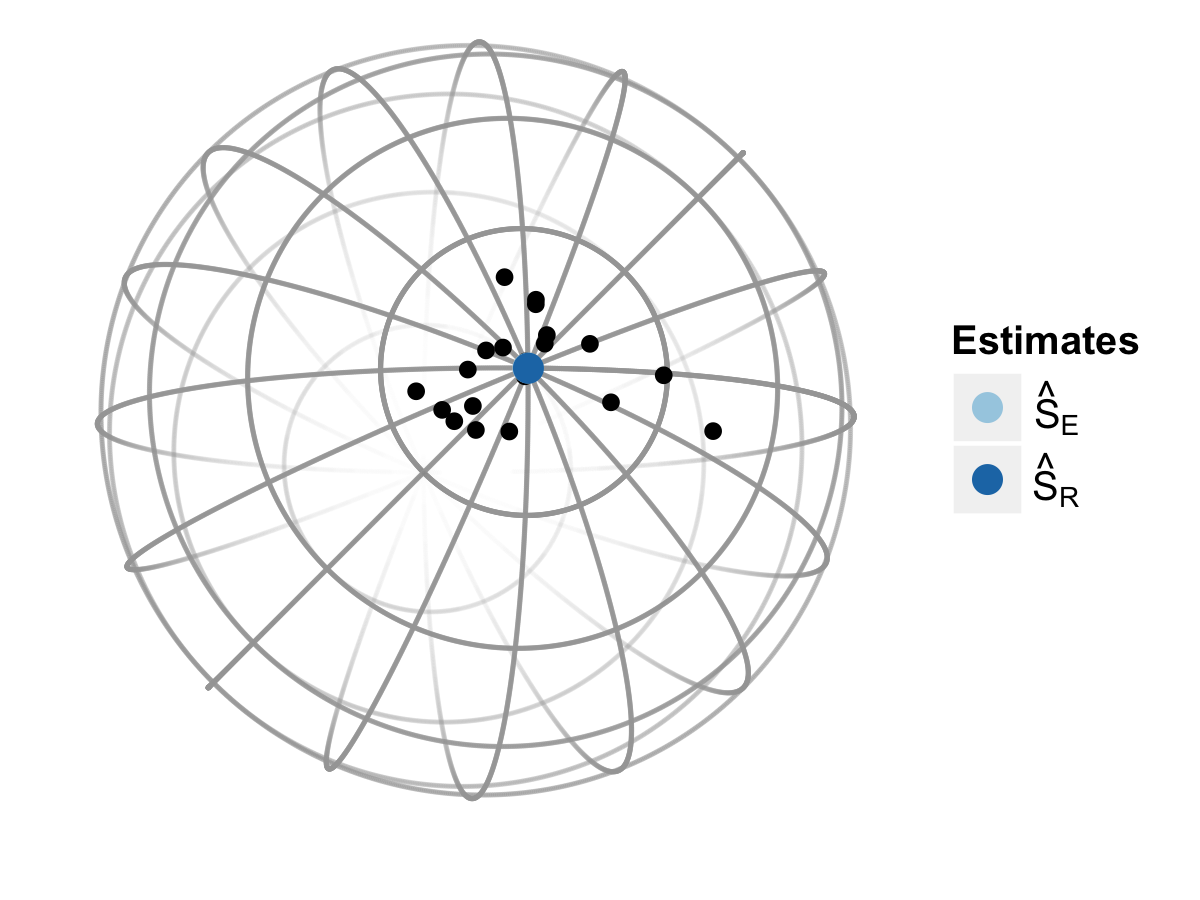
\includegraphics[width=\textwidth]{Figure/Sample1}
  \caption{}
  \label{fig:samp1}
\end{subfigure}
\begin{subfigure}[b]{0.45\textwidth}
  \centering
  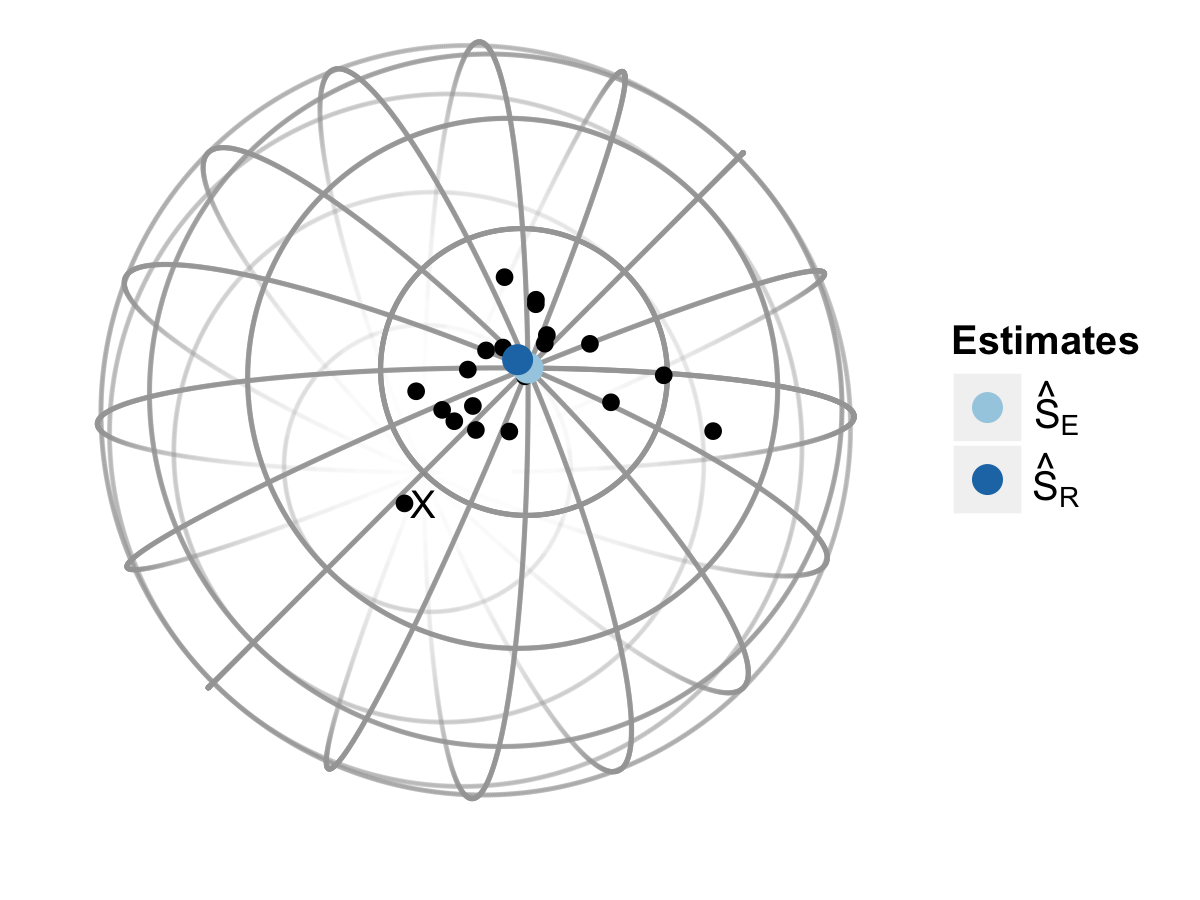
\includegraphics[width=\textwidth]{Figure/Sample2}
  \caption{}
  \label{fig:samp2}
\end{subfigure}
\caption{Random sample of size $20$ from Cayley($\bm I_{3\times 3},50$) distribution in (a).  Same sample with additional observation that is the rotation of $\ProjMean$ rotated through $\pi$ radians in (b), marked with an ``X".  Notice $\ProjMean$ is exactly the same in both samples, but $\GeomMean$ moves away.}
\label{fig:sample}
\end{figure}

The question as to which statistic is appropriate comes down to: why do you care?  Large $C$ statistic (and also influence function) values will determine which observation will have the largest impact on the projected mean estimate of center.  The $H_n$ statistic will tell you which observation is most unlike the others, but not necessarily the one that will impact estimation.

 
\section{Robustified Means}


To define the $SO(3)$ \emph{trimmed mean} we need to determine which observations are in the tails.  To do this consider the the discordant measure $H_i$ proposed by \cite{best1986} and later expanded to the hypersphere by \cite{figueiredo2005} defined in Section \ref{sec:outliers}.

It follows that $\alpha$-trimmed mean in $SO(3)$ is defined by
\[
\bm S_{T}=\frac{1}{|\Omega_0|}\int_{\Omega_0}\bm Rf(\bm R|\bm S,\kappa)d\bm R
\]
where $\Omega_0=\{\bm R:\bm R\in SO(3), H(\bm R)\leq q_{\alpha}\}$ and $q_\alpha$ is the $100(1-\alpha)\%$ of the distribution of $H_j$.  In practice $\bm S_T$ can be estimated by
\[
\TrimMean=\argmax_{\bm S\in SO(3)}\text{tr}(\bm S^\top\overline{\bm R}_T)
\]
where $\overline{\bm R}_T=\sum_{i=1}^n\bm R_iI(\bm H_i\leq \hat q_{\alpha})$ and $\hat q_{\alpha}$ is the $100(1-\alpha)\%$ of the distribution of $H_i$.


Define the $SO(3)$ \emph{weighted mean} as
\begin{align*}
\WeightMean=\argmax_{\bm S\in SO(3)}\text{tr}(\bm S^\top\overline{\bm R}_W)
\end{align*}
where $\overline{\bm R}_W=(\sum_{i}w_i\bm R_i)/(\sum_i w_i)$, the weights $w_i^{-1}=\sqrt{H_i}/(\sum_i \sqrt{H_i})$ and $H_i$ is from \eqref{eqn:Hj}.  I use the square root of $H_i$ because $H_i$ alone behaves like a square loss function instead of an absolute loss function.


The idea of the multidimensional \emph{Huber estimator} is to robustify an estimator by placing a bound on the norm of its influence function.  In Figure \ref{fig:Huber} the 2-dimensional case is illustrated for the artificial data $\bm q_1,\dots,\bm q_6$.
\begin{figure}
\begin{center}
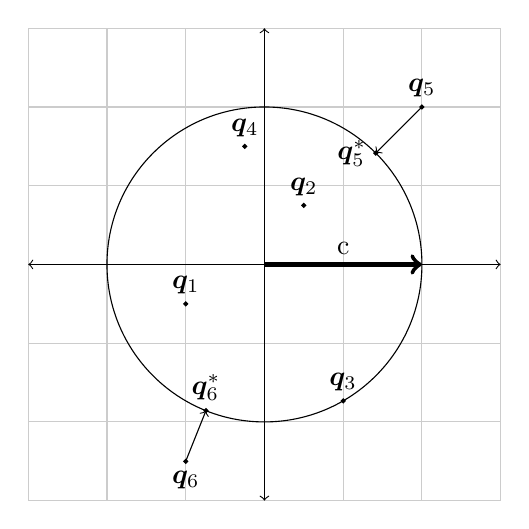
\begin{tikzpicture}
    \draw [black!20] (-3,-3) grid (3,3);
    \draw (0,0) circle [radius=2];
    \draw [->,ultra thick] (0,0) -- (2,0);
    \draw [<->] (-3,0) -- (3,0);
    \draw [<->] (0,-3) -- (0,3);
    %\node [above] at (3,0) {$x$}
    \node [above] at (1,0) {c};
    \node [above] at (-1,-.5) {$\bm{q}_1$};
    \draw [fill] (-1,-.5) circle [radius=0.025];
    \node [above] at (.5,.75) {$\bm{q}_2$};
    \draw [fill] (.5,.75) circle [radius=0.025];
    \node [above] at (1,-1.732051) {$\bm{q}_3$};
    \draw [fill] (1,-1.732051) circle [radius=0.025];
    \node [above] at (-.25,1.5) {$\bm{q}_4$};
    \draw [fill] (-.25,1.5) circle [radius=0.025];
    \node [above] at (2,2) {$\bm{q}_5$};
    \draw [fill] (2,2) circle [radius=0.025];
    \node [left] at (1.414214, 1.414214) {$\bm{q}_5^*$};
    \draw [fill] (1.414214, 1.414214) circle [radius=0.025];
    \draw [->] (2,2) -- (1.414214, 1.414214);
    \node [below] at (-1,-2.5) {$\bm{q}_6$};
    \draw [fill] (-1,-2.5) circle [radius=0.025];
    \node [above] at (-0.7427814,  -1.8569534) {$\bm{q}_6^*$};
    \draw [fill] (-0.7427814, -1.8569534) circle [radius=0.025];
    \draw [->] (-1,-2.5) -- (-0.7427814,  -1.8569534);
\end{tikzpicture}
\end{center}
\caption{Multidimensional Huber estimator as illustrated in Section 4.3 of \cite{hampel2011}.}
\label{fig:Huber}
\end{figure}

Each point represents the influence function evaluated at that data point.  The norm of the influence function for this estimator evaluated at $\bm q_1,\dots,\bm q_4$ all lie within the specified distance of the origin so they are left untouched.  The norm of the influence function evaluated at $\bm q_5$ and $\bm q_6$ however is larger than $c$ and therefore those points are altered such that the norm of the influence function has a norm of $c$.  The reason (according to pp 239 of \citealt{hampel2011}) for placing the bound on the influence function is because  ``the most meaningful version of the $\psi$-function defining an $M$-estimator is its influence function."

Applying this idea to $SO(3)$ data, recall from the regions paper that the influence function of $\ProjMean$ is
\[
\text{IF}_2(\bm R_i,F)=\frac{3}{1+2E[\cos(r)]}\sin(r)\bm u
\]
where $r=d_r(\bm R_i,\bm S)$ or in practice $\hat{r}=d_r(\bm R_i,\ProjMean)$.  It follows that $\|\text{IF}_2(\bm R_i,F)\|\propto \sin(|r|)$.  Unfortunately, using the Huber estimator directly will put the most restrictions on the $r$ values near $\pi/2$ instead or $\pi$, which is where we really want to place the upper bound.  Therefore I propose the modified Huber estimator on $SO(3)$ put a bound on $r_i=d_r(\bm R_i,\ProjMean)$ and is denoted $\HuberMean$.  

The algorithm I use to compute $\HuberMean$ based on the sample $\bm R_1,\dots,\bm R_n$ and the constant $c<\pi$ is as follows
\begin{enumerate} 
\item Compute $\ProjMean^{(j)}$
\item For each $i$ compute $r_i^{(j)}=d_r(\bm R_i,\ProjMean^{(j)})$
\item For each $i$ such that $r_i>c$:
\begin{enumerate}
\item Find $\bm u_i\in\mathcal{S}^3$ satisfying $\exp[\bm{\Phi}(r_i\bm u_i)]=\ProjMean^{(j)\top}\bm R_i$
\item Redefine $\bm R_i=\ProjMean^{(j)\top}\exp[\bm{\Phi}(c\bm u_i)]$
\end{enumerate}
\item Repeat steps 1 - 3 for $j+1$ until $r_i<c$ for all $i$
\item Define $\HuberMean=\ProjMean^{(j+1)}$
\end{enumerate}

The \emph{winsorized mean} is a combination of the trimmed mean and winsorized mean.  That is, the data are ordered according to their respective $H_j$ values.  All rotations beyond the upper $100(1-\alpha)$\% percentage is projected to the border of the inner circle while maintaining the original axis of rotation.  The mathematical definition is 
\[
\WinzMean=\argmax_{\bm S\in SO(3)}\text{tr}(\bm S^\top\overline{\bm R}_{Z})
\]
where $\overline{\bm R}_{Z}=\sum_{i=1}^n\bm R_i^*/n$, 
\[
\bm R_i^*=
\begin{cases}
\bm R_i&\text{ if }d_R(\ProjMean,\bm R_i)\leq\hat{q}\\
\ProjMean\exp[\bm{\Phi}(\hat{q}\bm{u}_i^*)]&\text{ otherwise,}
\end{cases}
\]
$\bm u_i^*$ is the axis of rotation corresponding to $\ProjMean^\top\bm R_i$ and $\hat{q}$ is the $100(1-\alpha)$\% percentile of the distribution of $H_j$.




\section{(Very) Limited Simulation Study}

I ran a very small simulation study with the new robustified $\ProjMean$ estimators (trimmed, winsorized, weighted, Huber) along with the tradition $\ProjMean$ and $\ProjMedian$.  I generated 100 samples per combination of distribution (Cayley or von Mises Fisher), sample size ($n=10,50$), concentration ($\kappa=0.5,1,10$) all with $10\%$ contamination.  Meaning 90\% of each sample was from the $F(\bm I_{3\times 3},\kappa)$ distribution and 10\% of the sample came from a $F(\bm S_c[\pi/2,\bm u],\kappa)$, i.e.~the slippage situation where the second principal direction was rotation though $\pi/2$ radians about some (uniformly distributed) axis.

In Table \ref{tab:SimResHn} is the average bias based on the Euclidean distance in each estimator for each simulated scenario.  That is bias$=\|\bm I_{3\times 3}-\widehat{\bm S}\|_F$ for each estimator.  The trimmed and winsorized mean use $\alpha=0.1$ and the Huber estimator sets $c=0.75$.




\begin{table}[ht]
\centering
\begin{tabular}{l|lll|lll|lll|lll}
  \hline
 & \multicolumn{6}{|c|}{Cayley} & \multicolumn{6}{|c}{von Mises}   \\ 
\hline
   &  \multicolumn{3}{|c|}{n=10} & \multicolumn{3}{|c|}{n=50} & \multicolumn{3}{|c|}{n=10} & \multicolumn{3}{|c}{n=50} \\ 
  $\kappa$ &  0.5 &  1.0 & 10.0 &  0.5 &  1.0 & 10.0 &  0.5 &  1.0 & 10.0 &  0.5 &  1.0 & 10.0 \\ \hline
  $\ProjMedian$ (Median) & 1.71 & 1.30 & 0.37 & 0.92 & 0.66 & 0.18 & 0.52 & 0.33 & 0.09 & 0.15 & 0.11 & 0.03 \\ 
  $\ProjMean$ (Mean) & 1.55 & 1.10 & 0.35 & 0.79 & 0.55 & 0.21 & 0.66 & 0.49 & 0.20 & 0.31 & 0.23 & 0.17 \\ 
  $\TrimMean$ (Trim) & 1.56 & 1.16 & 0.34 & 0.80 & 0.57 & 0.16 & 0.70 & 0.52 & 0.13 & 0.33 & 0.24 & 0.06 \\ 
  $\WinzMean$ (Winsorize)& 1.56 & 1.11 & 0.36 & 0.75 & 0.51 & 0.21 & 0.68 & 0.51 & 0.18 & 0.32& 0.24 & 0.12 \\ 
  $\WeightMean$ (Weight) & 1.61 & 1.17 & 0.36 & 0.84 & 0.60 & 0.19& 0.56 & 0.39 & 0.12 & 0.21 & 0.15 & 0.07\\ 
  $\HuberMean$ (Huber) & 1.55 & 1.11 & 0.35 & 0.77 & 0.54 & 0.20 & 0.65 & 0.47 & 0.17 & 0.30 & 0.22 & 0.13 \\ 
   \hline
\end{tabular}
\caption{Mean estimator bias based on 100 samples from each combination of distribution, sample size and concentration.  The robustified $L_2$ estimator is based on the distance of the observations from the bulk of the data, quantified by the $H_n$ statistic.}
\label{tab:SimResHn}
\end{table}

\begin{table}[ht]
\centering
\begin{tabular}{l|lll|lll|lll|lll}
  \hline
 & \multicolumn{6}{|c|}{Cayley} & \multicolumn{6}{|c}{von Mises}   \\ 
\hline
   &  \multicolumn{3}{|c|}{n=10} & \multicolumn{3}{|c|}{n=50} & \multicolumn{3}{|c|}{n=10} & \multicolumn{3}{|c}{n=50} \\
  $\kappa$ &  0.5 &  1.0 & 10.0 &  0.5 &  1.0 & 10.0 &  0.5 &  1.0 & 10.0 &  0.5 &  1.0 & 10.0 \\ \hline
  $\ProjMedian$ (Median) & 1.70 & 1.25 & 0.35 & 1.01 & 0.59 & 0.19 & 0.55 & 0.37 & 0.08 & 0.15 & 0.11 & 0.03 \\ 
  $\ProjMean$ (Mean) & 1.56 & 1.04 & 0.33 & 0.83 & 0.49 & 0.22 & 0.76 & 0.50 & 0.19 & 0.30 & 0.25 & 0.17 \\ 
   $\TrimMean$ (Trim) & 1.68 & 1.12 & 0.34 & 0.86 & 0.52 & 0.17 & 0.82 & 0.53 & 0.13 & 0.31 & 0.23 & 0.06 \\ 
  $\WinzMean$ (Winsorize) & 1.60 & 1.06 & 0.34 & 0.82 & 0.49 & 0.18 & 0.74 & 0.51 & 0.13 & 0.29 & 0.22 & 0.06 \\ 
  $\WeightMean$ (Weight) & 2.07 & 1.52 & 0.33 & 2.06 & 0.83 & 0.20 & 1.37 & 0.74 & 0.12 & 0.75 & 0.41 & 0.08 \\ 
  $\HuberMean$ (Huber) & 1.56 & 1.03 & 0.33 & 0.82 & 0.48 & 0.20 & 0.74 & 0.49 & 0.16 & 0.28 & 0.23 & 0.13 \\ 
   \hline
\end{tabular}
\caption{Mean estimator bias based on 100 samples from each combination of distribution, sample size and concentration.  The robustified $L_2$ estimator is based on the influence of the point on the $L_2$ estimator, quantified by the influence function.}
\label{tab:SimResC}
\end{table}


% \begin{figure}
% \centering
% 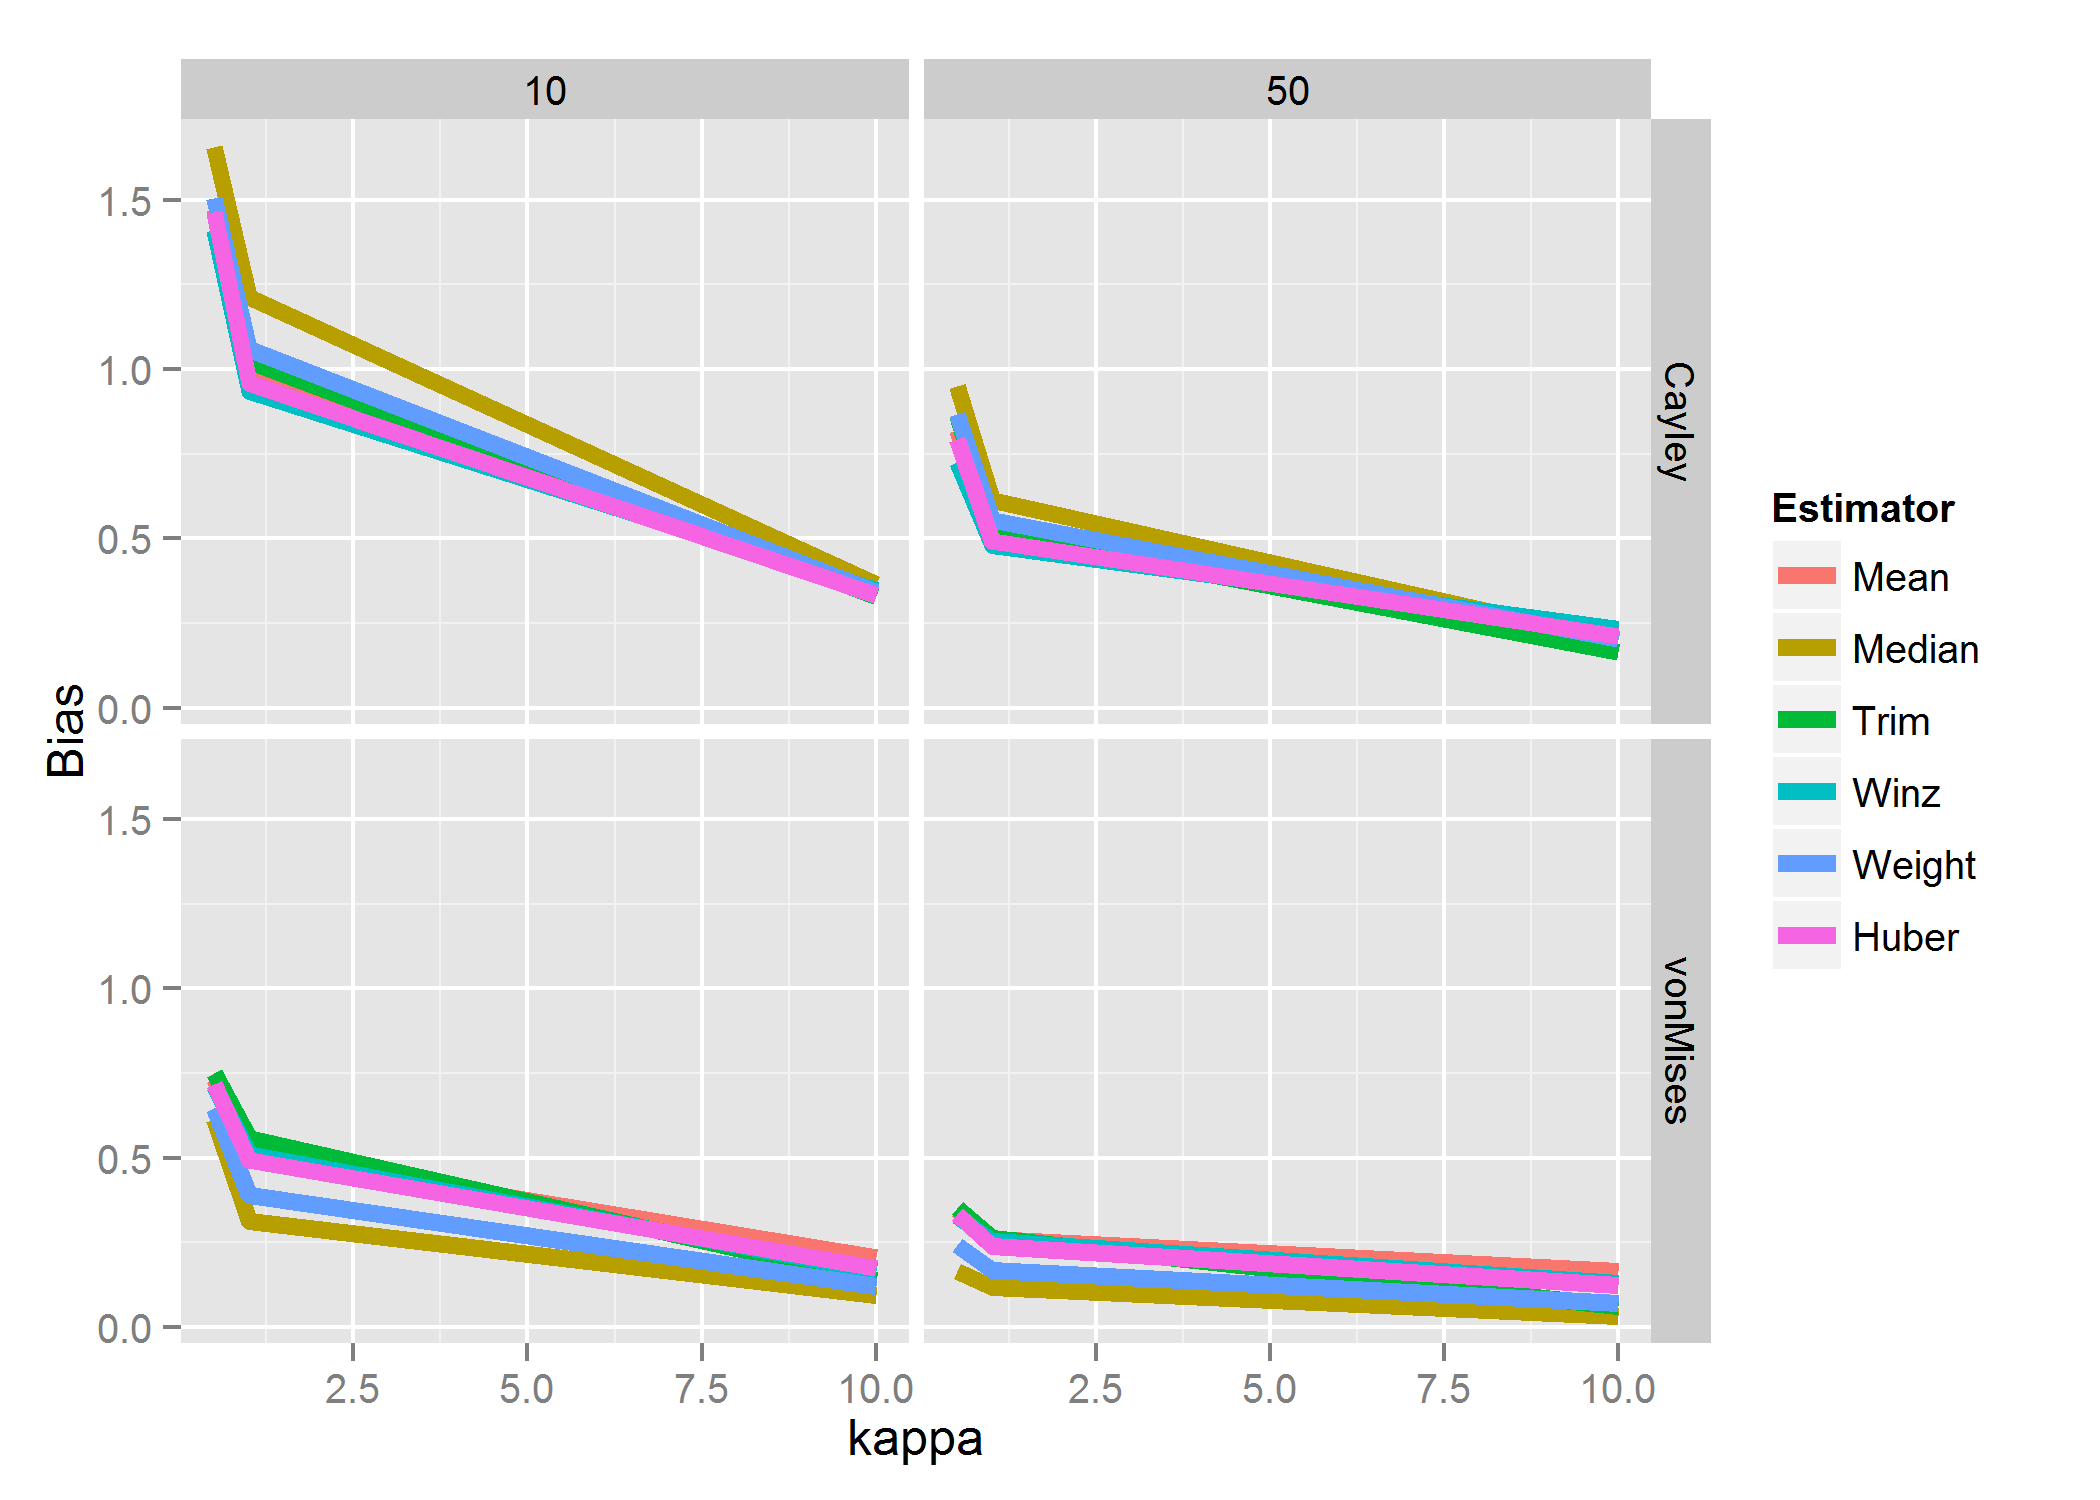
\includegraphics[width=.7\textwidth]{Estimator.png}
% \caption{Graphical representation of Table \ref{tab:SimResHn} faceted by sample size and distribution.}
% \end{figure}


For the Cayley (and presumably Fisher matrix) distribution, the Huber estimator and trimmed mean are close.  Trimmed mean is preferred for more concentrated data and the Huber estimator is preferred as the data become less concentrated.  This makes sense because the trimmed mean is discarding the contaminated data when the bulk of the data is highly concentrated, while the Huber estimator is trying to use all the data.  The median does really poorly, even compared to the mean.

For the von Mises distribution, it looks like the median is unbeatable.  This is likely due to the heavy tail we identified in the Technometrics paper.  Similar to the other distribution, the trimmed mean improves considerably as the bulk of the data becomes more concentrated and the contamination can be cut out completely.  The Huber estimator and winsorized mean give comparable results but are not terribly good.
\clearpage
%\bibliographystyle{plain}
\bibliography{../OutlierDetection/RobustRefs}
\end{document}
